\documentclass[agums,grl]{agutexSI}

%% -----------------------

\usepackage{xcolor}
\usepackage[letterpaper]{geometry}
\usepackage{draftwatermark}
\SetWatermarkText{Draft}
\SetWatermarkScale{5}

\usepackage{graphicx}
\graphicspath{ {figures/} }

\usepackage{lineno}
\linenumbers*[1]
\setlength{\columnsep}{25pt}

%% ------------------------------------------------------------------------ %%
%
%  ENTER PREAMBLE
%
%% ------------------------------------------------------------------------ %%

% Author names in capital letters:
\authorrunninghead{GRIMA ET AL.}

% Shorter version of title entered in capital letters:
\titlerunninghead{BRINE EXTENT AT MCMURDO ICE SHELF}

%Corresponding author mailing address and e-mail address:
\authoraddr{Corresponding author: C. Grima,
Institute for Geophysics, J.J. Pickle Research Campus, Bldg. 196, 10100 Burnet Rd. (R2200), Austin, TX 78758-4445, USA
(cyril.grima@gmail.com)}


\begin{document}

%% ------------------------------------------------------------------------ %%
%
%  TITLE
%
%% ------------------------------------------------------------------------ %%


\title{Supporting Information for ``Brine extent at McMurdo Ice Shelf, Antarctica, controlled by snow accumulation"}

DOI: 10.1002/%insert paper number here%

%% ------------------------------------------------------------------------ %%
%
%  AUTHORS AND AFFILIATIONS
%
%% ------------------------------------------------------------------------ %%

\authors{Cyril Grima,\altaffilmark{1}
Jamin S. Greenbaum,\altaffilmark{1} Erika J. Lopez Garcia,\altaffilmark{1}
Krista M. Soderlund,\altaffilmark{1} Donald D. Blankenship,\altaffilmark{1} and Duncan A. Young\altaffilmark{1}}

\altaffiltext{1}{Institute for Geopysics, University of Texas at Austin, TX 78758, USA.}

%% ------------------------------------------------------------------------ %%
%
%  BEGIN ARTICLE
%
%% ------------------------------------------------------------------------ %%

\begin{article}

%% ------------------------------------------------------------------------ %%
%
%  TEXT
%
%% ------------------------------------------------------------------------ %%



\noindent\textbf{Contents of this file}
%%%Remove or add items as needed%%%
\begin{enumerate}
\item Radar Statistical Reconnaissance over McMurdo Ice Shelf
\item Reflectance
\item Scattering
\item Correlation Coefficient ($\rho$)
\item Root-Mean-Square Height ($\sigma_h$)
\item Permittivity ($\epsilon$)
\end{enumerate}

\vspace{5 mm}

\noindent\textbf{Introduction}
The supplementary materials include detailed explanations for the Radar Statistical Reconnaissance principles and applications with the HiCARS2 data set from the 2011-2012 austral summer survey over McMurdo Ice Shelf (MIS). Figures illustrating the RSR results are also provided.

\vspace{5 mm}

\noindent\textbf{Text S1. Radar Statistical Reconnaissance over McMurdo Ice Shelf}

We have used the Radar Statistical Reconnaissance (RSR) in the same manner as \citet{Grima-2014-ID865,Grima-2014-ID867} to derive the root-mean-square heights ($\sigma_h$) and surface snow density ($d$) over Thwaites glacier, West Antarctica, with HiCARS data. In the MIS case, the along-track data are divided into 1-km sampled spaces ($\sim$1000 surface echoes) repeated every 250~m. The RSR is applied on every sampled space to derive their own set of signal components pair and surface properties.
The echo amplitude distributions are fitted with Homodyned K-statistics (HK) that allows the scatterers' amount to be few (non-fully developed speckle) or many (fully-developed speckle) and to be clustered within a footprint (non-stationary) \citep{Jakeman-1980-ID344,Jakeman-1987-ID343}. Signal reflectance (Fig.~\ref{pcpn}.top) and scattering (Fig.~\ref{pcpn}.bottom) are parameters of the HK envelope and are obtained from the best fit. The correlation coefficient ($\rho$, Fig. \ref{correlcoef}) of the fit is a qualitative confidence factor to estimate the terrain level-of-compliance with the statistical assumptions.
\par
$\sigma_h$ (Fig.~\ref{roughness}) and $\epsilon$ (Fig.~\ref{permittivity}) are then inverted from the Small Perturbation Model (SPM) \citep[e.g.][]{Ulaby-1981-ID816,Ogilvy-1991-ID817} with the additional assumption of a footprint-size or higher correlation length for the roughness. The SPM is valid only when $\sigma_h = 0.05 \lambda$ (error~$<$~1~dB; $\lambda$ is radar wavelength) \citep{Thorsos-1989-ID713}, i.e. $\sigma_h$~=~0.25~m for HiCARS2 over a horizontal scale of few wavelengths [Grima et al., 2014a]. These assumptions have been tested and validated over Thwaites Glacier, West Antarctica, using laser altimetry measurements.
\par
% Fig. \ref{density} seems to be missing in two spots in this paragraph.
$\epsilon$ is then translated into dry-snow density ($d$) from an empirical relationship \citep{Kovacs-1995-ID697,Frolov-1999-ID216}. In a steady-state accumulation model, the obtained radar-derived density can be considered as a value for the very top surface (depth~$\approx$~0~m) \citep{Grima-2014-ID867}. The radar signal has been calibrated over the known ablation area, West of Pegasus airfield, by adjusting the RSR-derived density there to that of solid ice (917~kg.m$^{-3}$) \citep{Frolov-1999-ID216}. The exact calibration location (E309009, N-1276517) (red diamond on Fig.~\ref{pt}-\ref{permittivity}) corresponds to a high reflectivity spot combined with $\rho=$~99.0~\%.

\end{article}


\newpage


 \begin{figure}
\setfigurenum{S2} %%Change number for each figure
 \noindent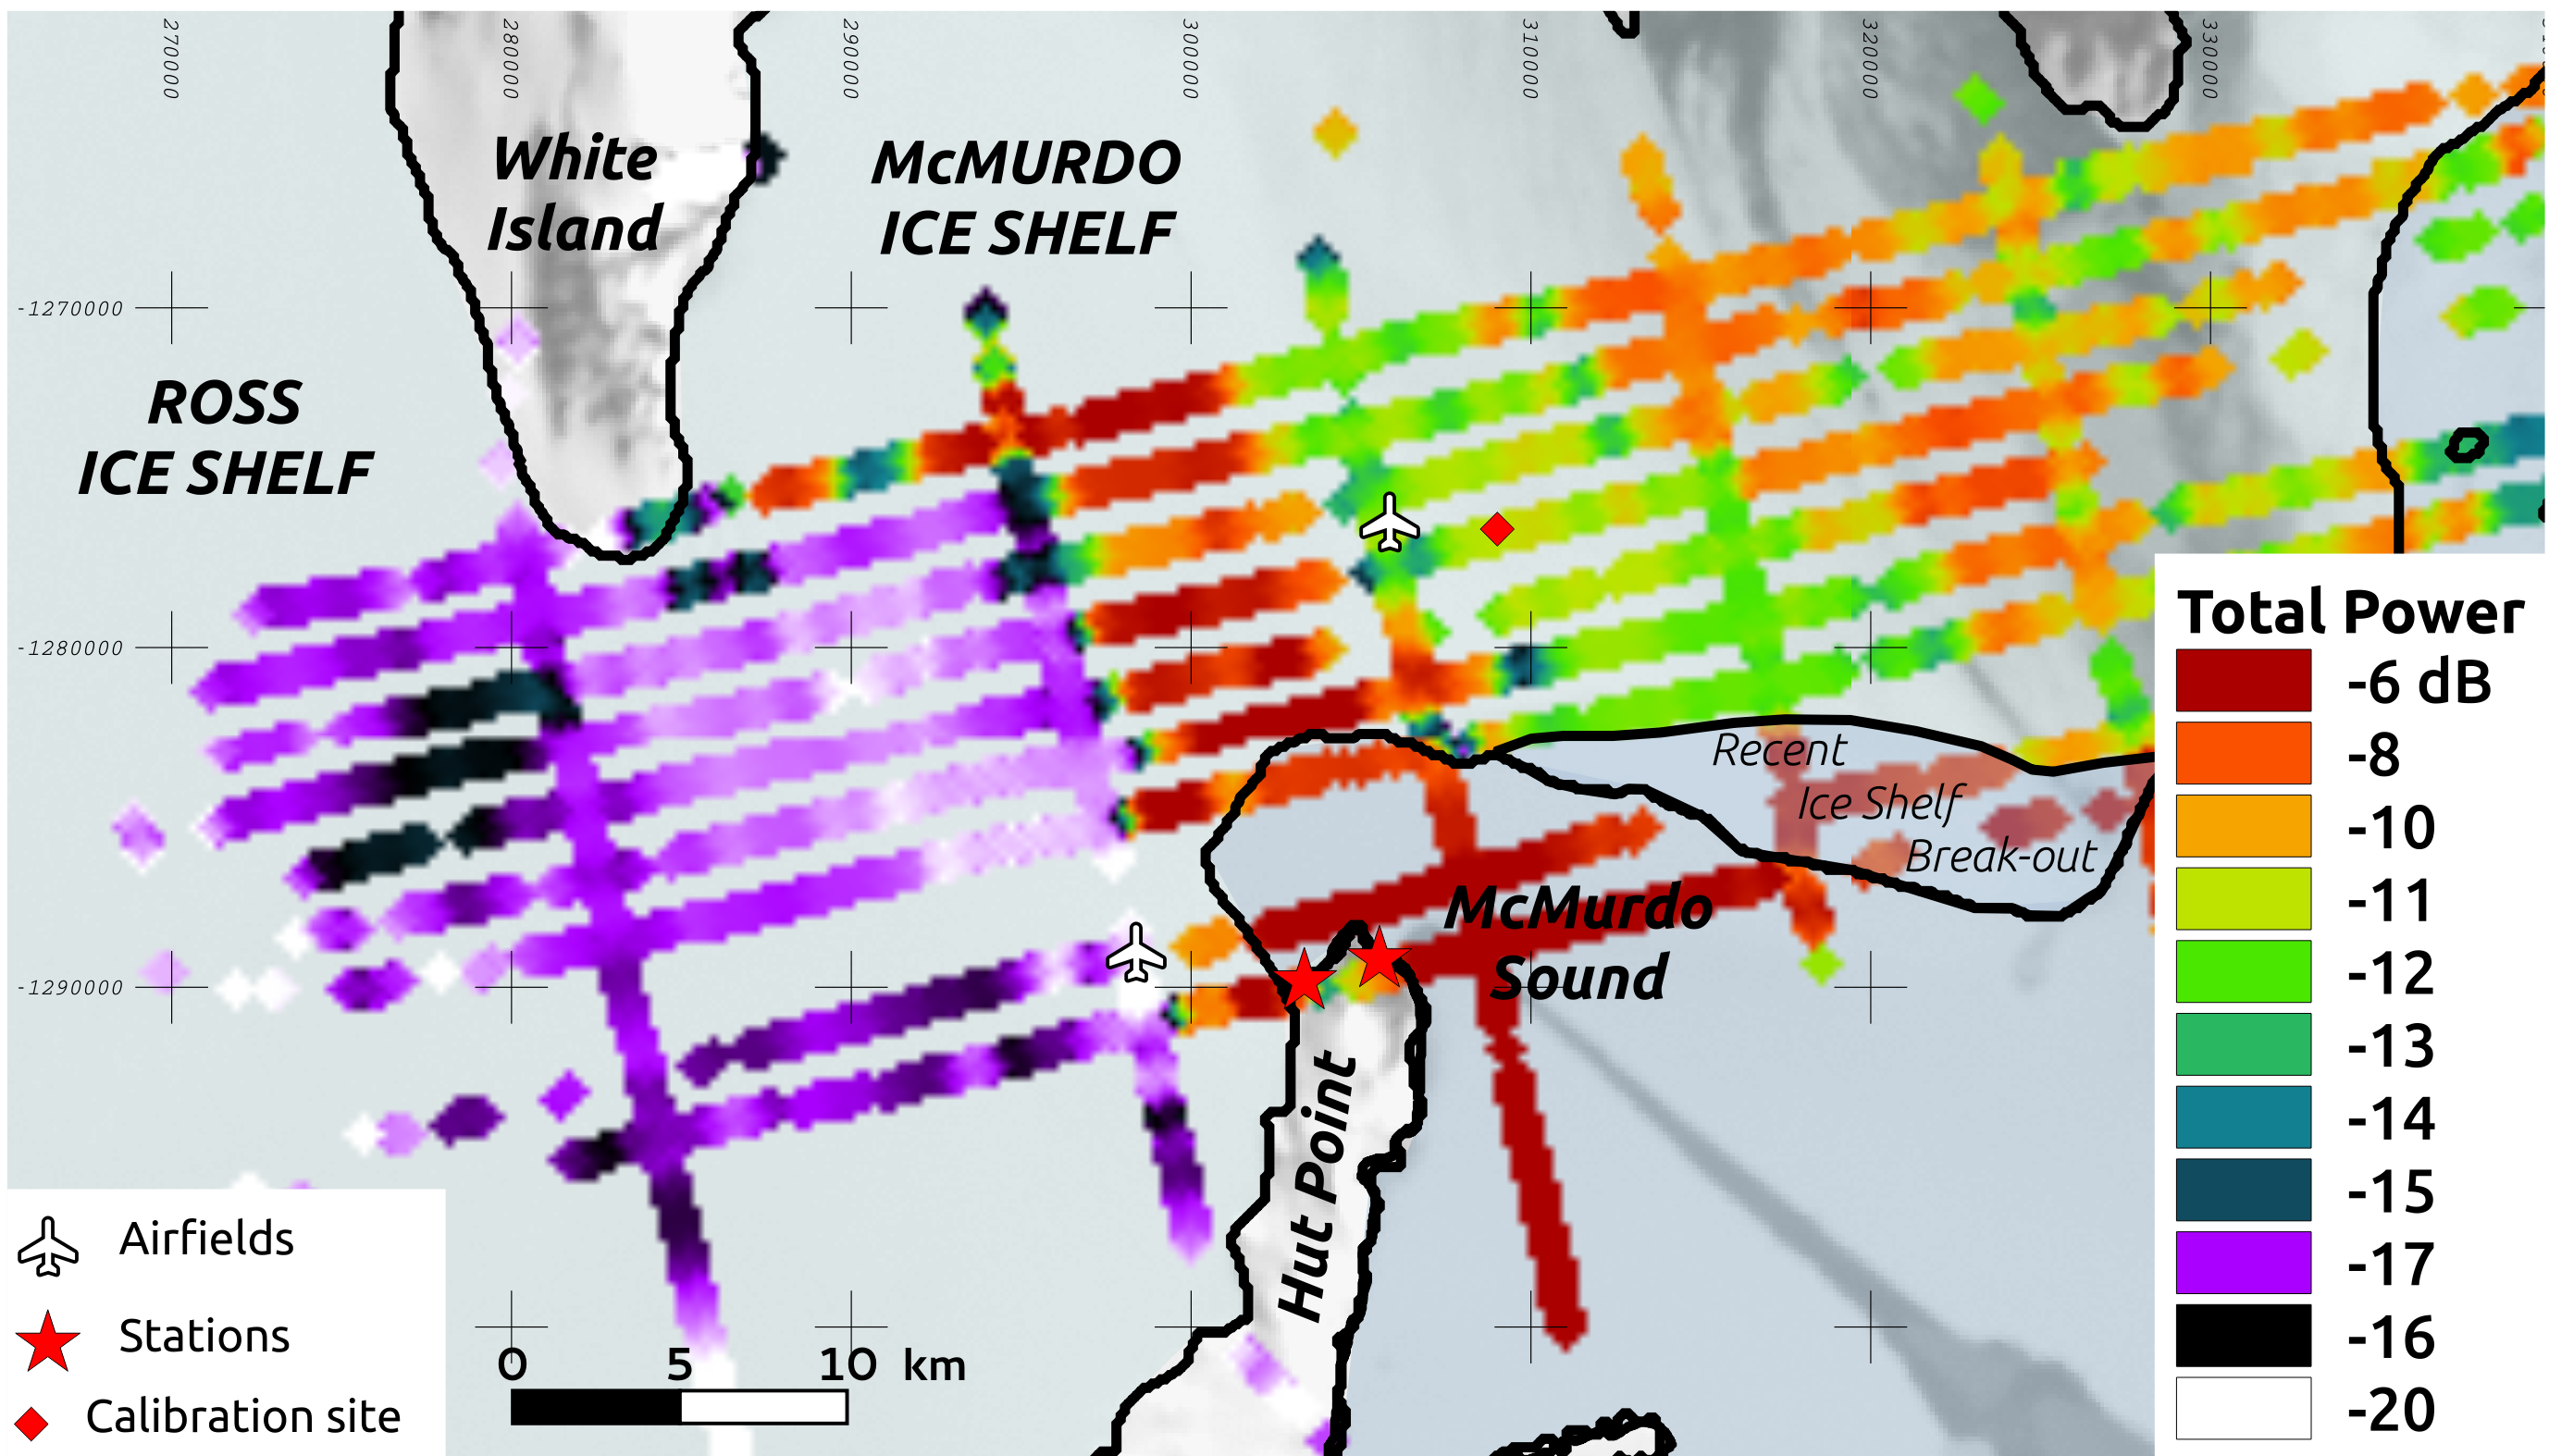
\includegraphics[width=\textwidth]{figS2}
\caption{Total signal power of the HiCARS2 surface echo. The signal is adjusted so that a reflection over a perfect mirror would be 0 dB (no loss). This is the surface signal used by the RSR to derive surface properties.}
 \label{pt}
 \end{figure}


 \begin{figure}
\setfigurenum{S3}  %%Change number for each figure
 \noindent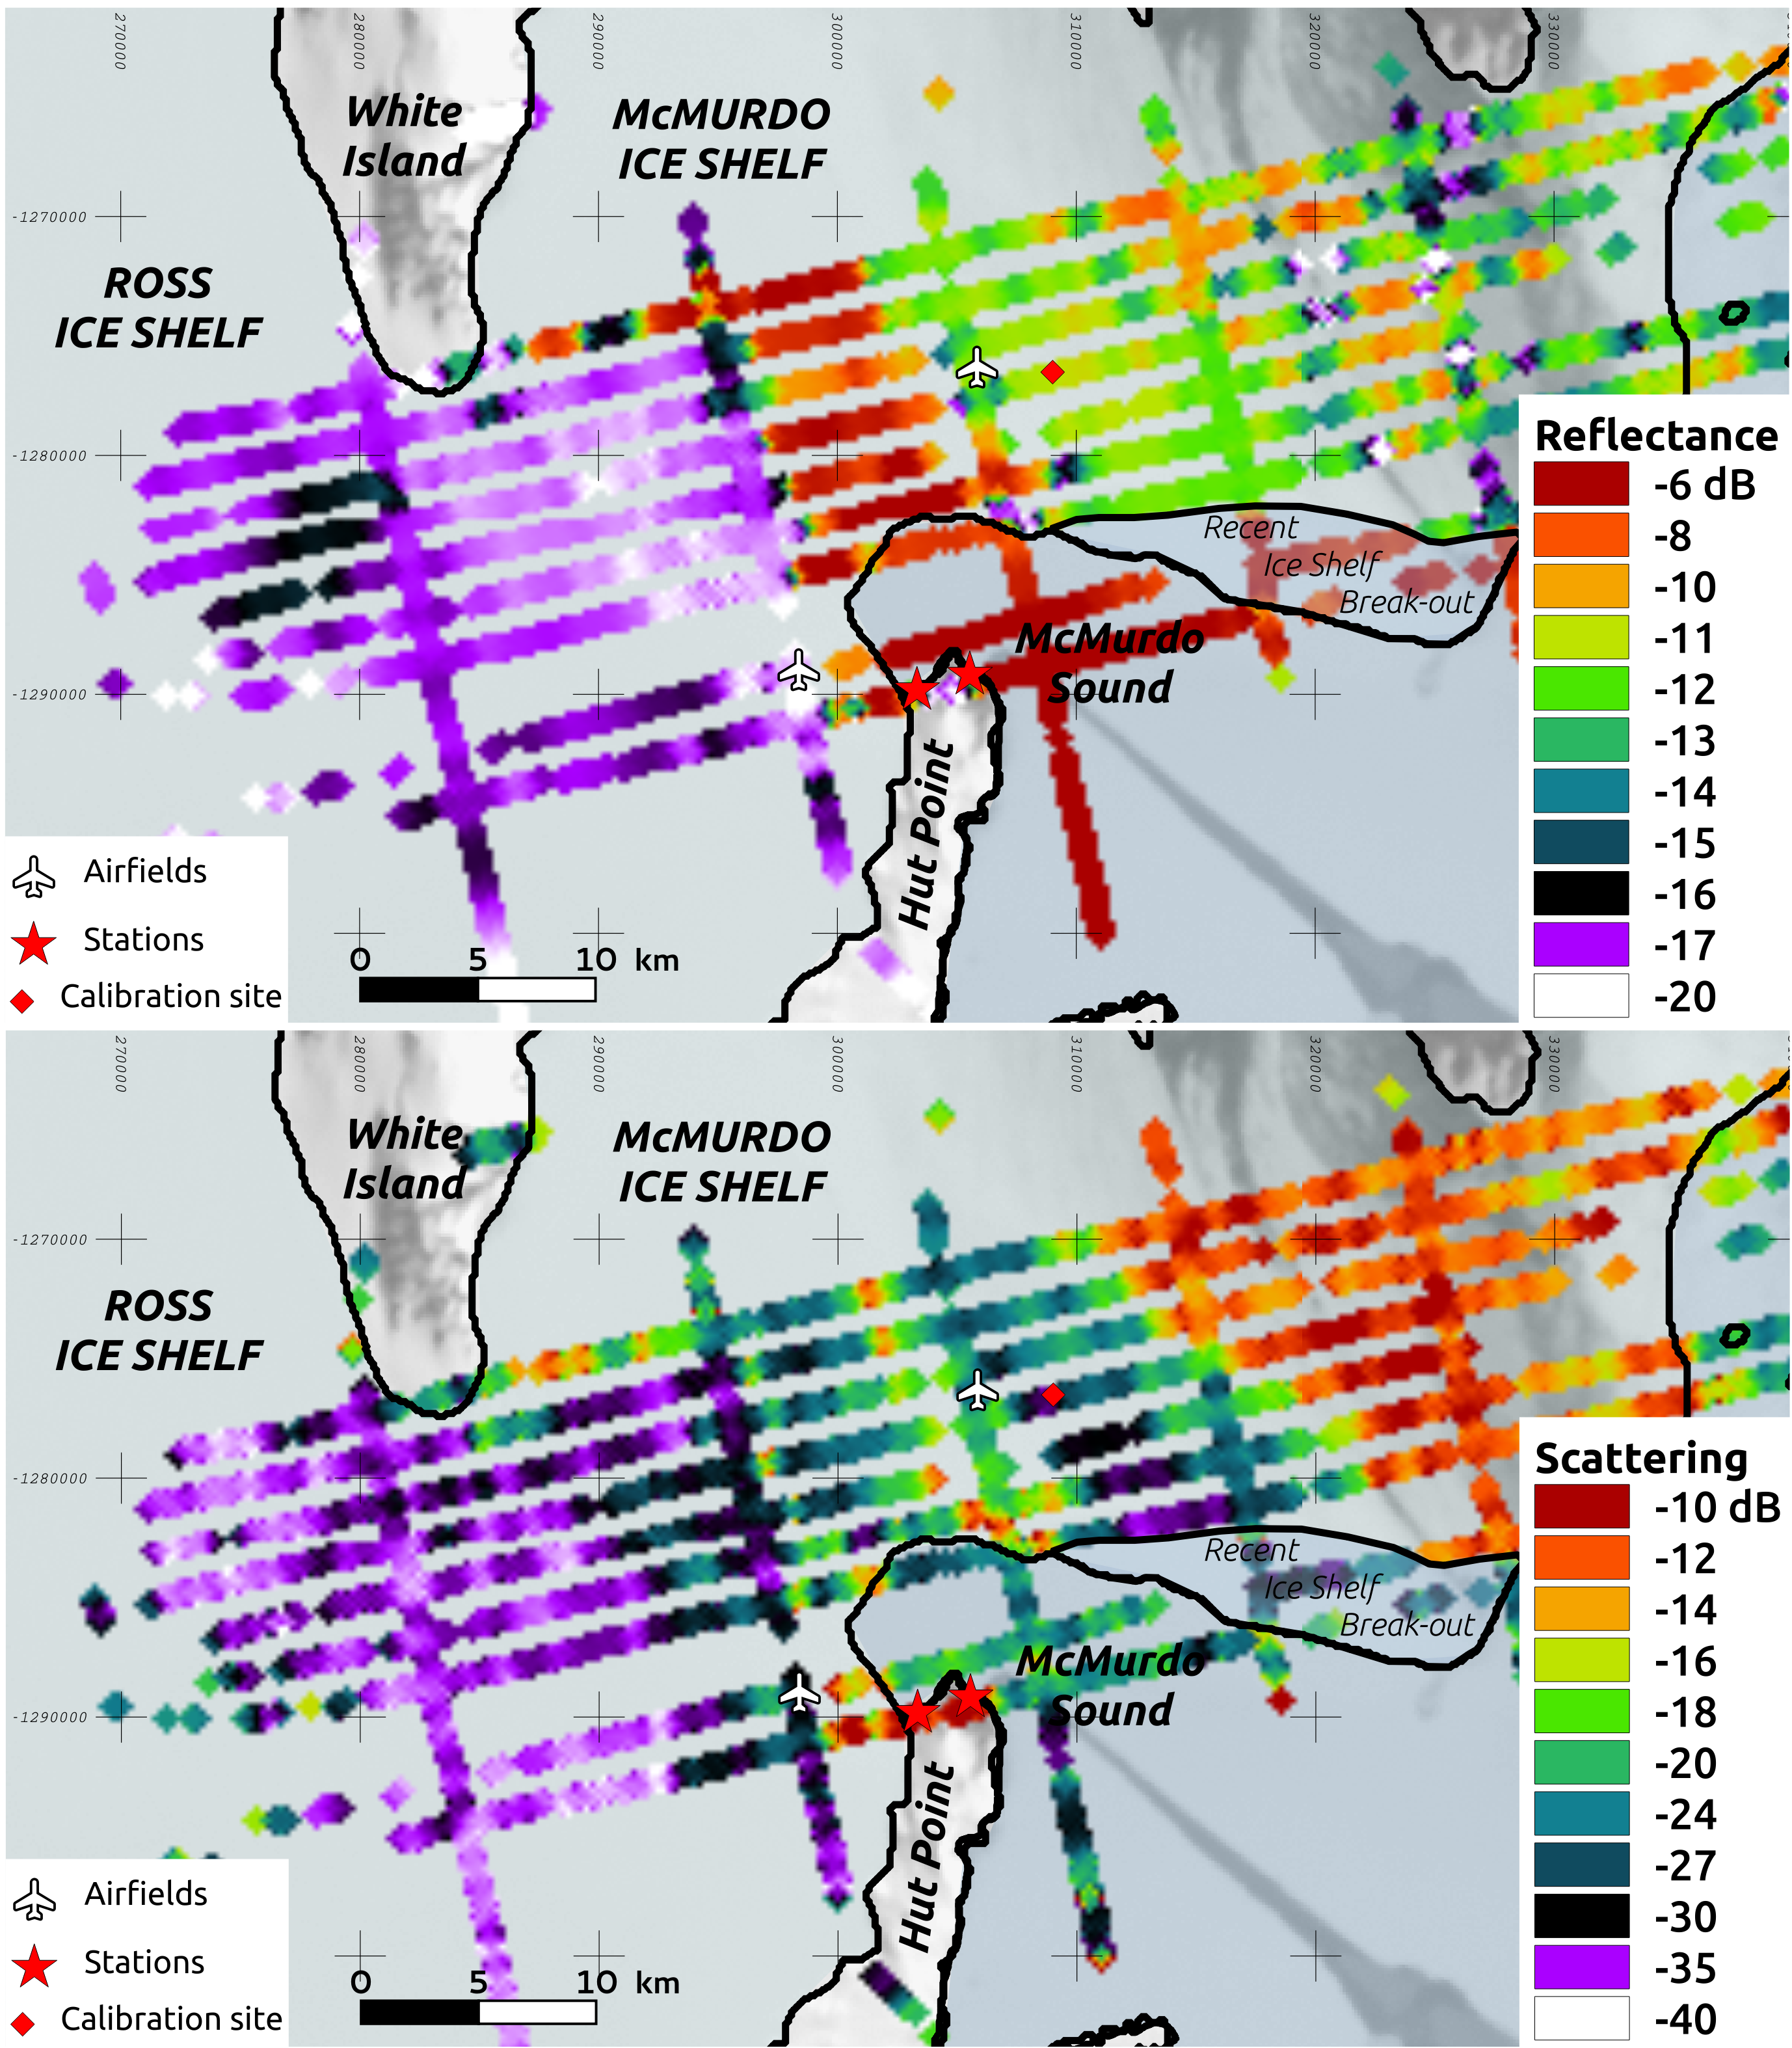
\includegraphics[width=\textwidth]{figS3}
\caption{Surface reflectance (top) and scattering (bottom) derived from RSR.}
 \label{pcpn}
 \end{figure}
 
 
  \begin{figure}
\setfigurenum{S4}  %%Change number for each figure
 \noindent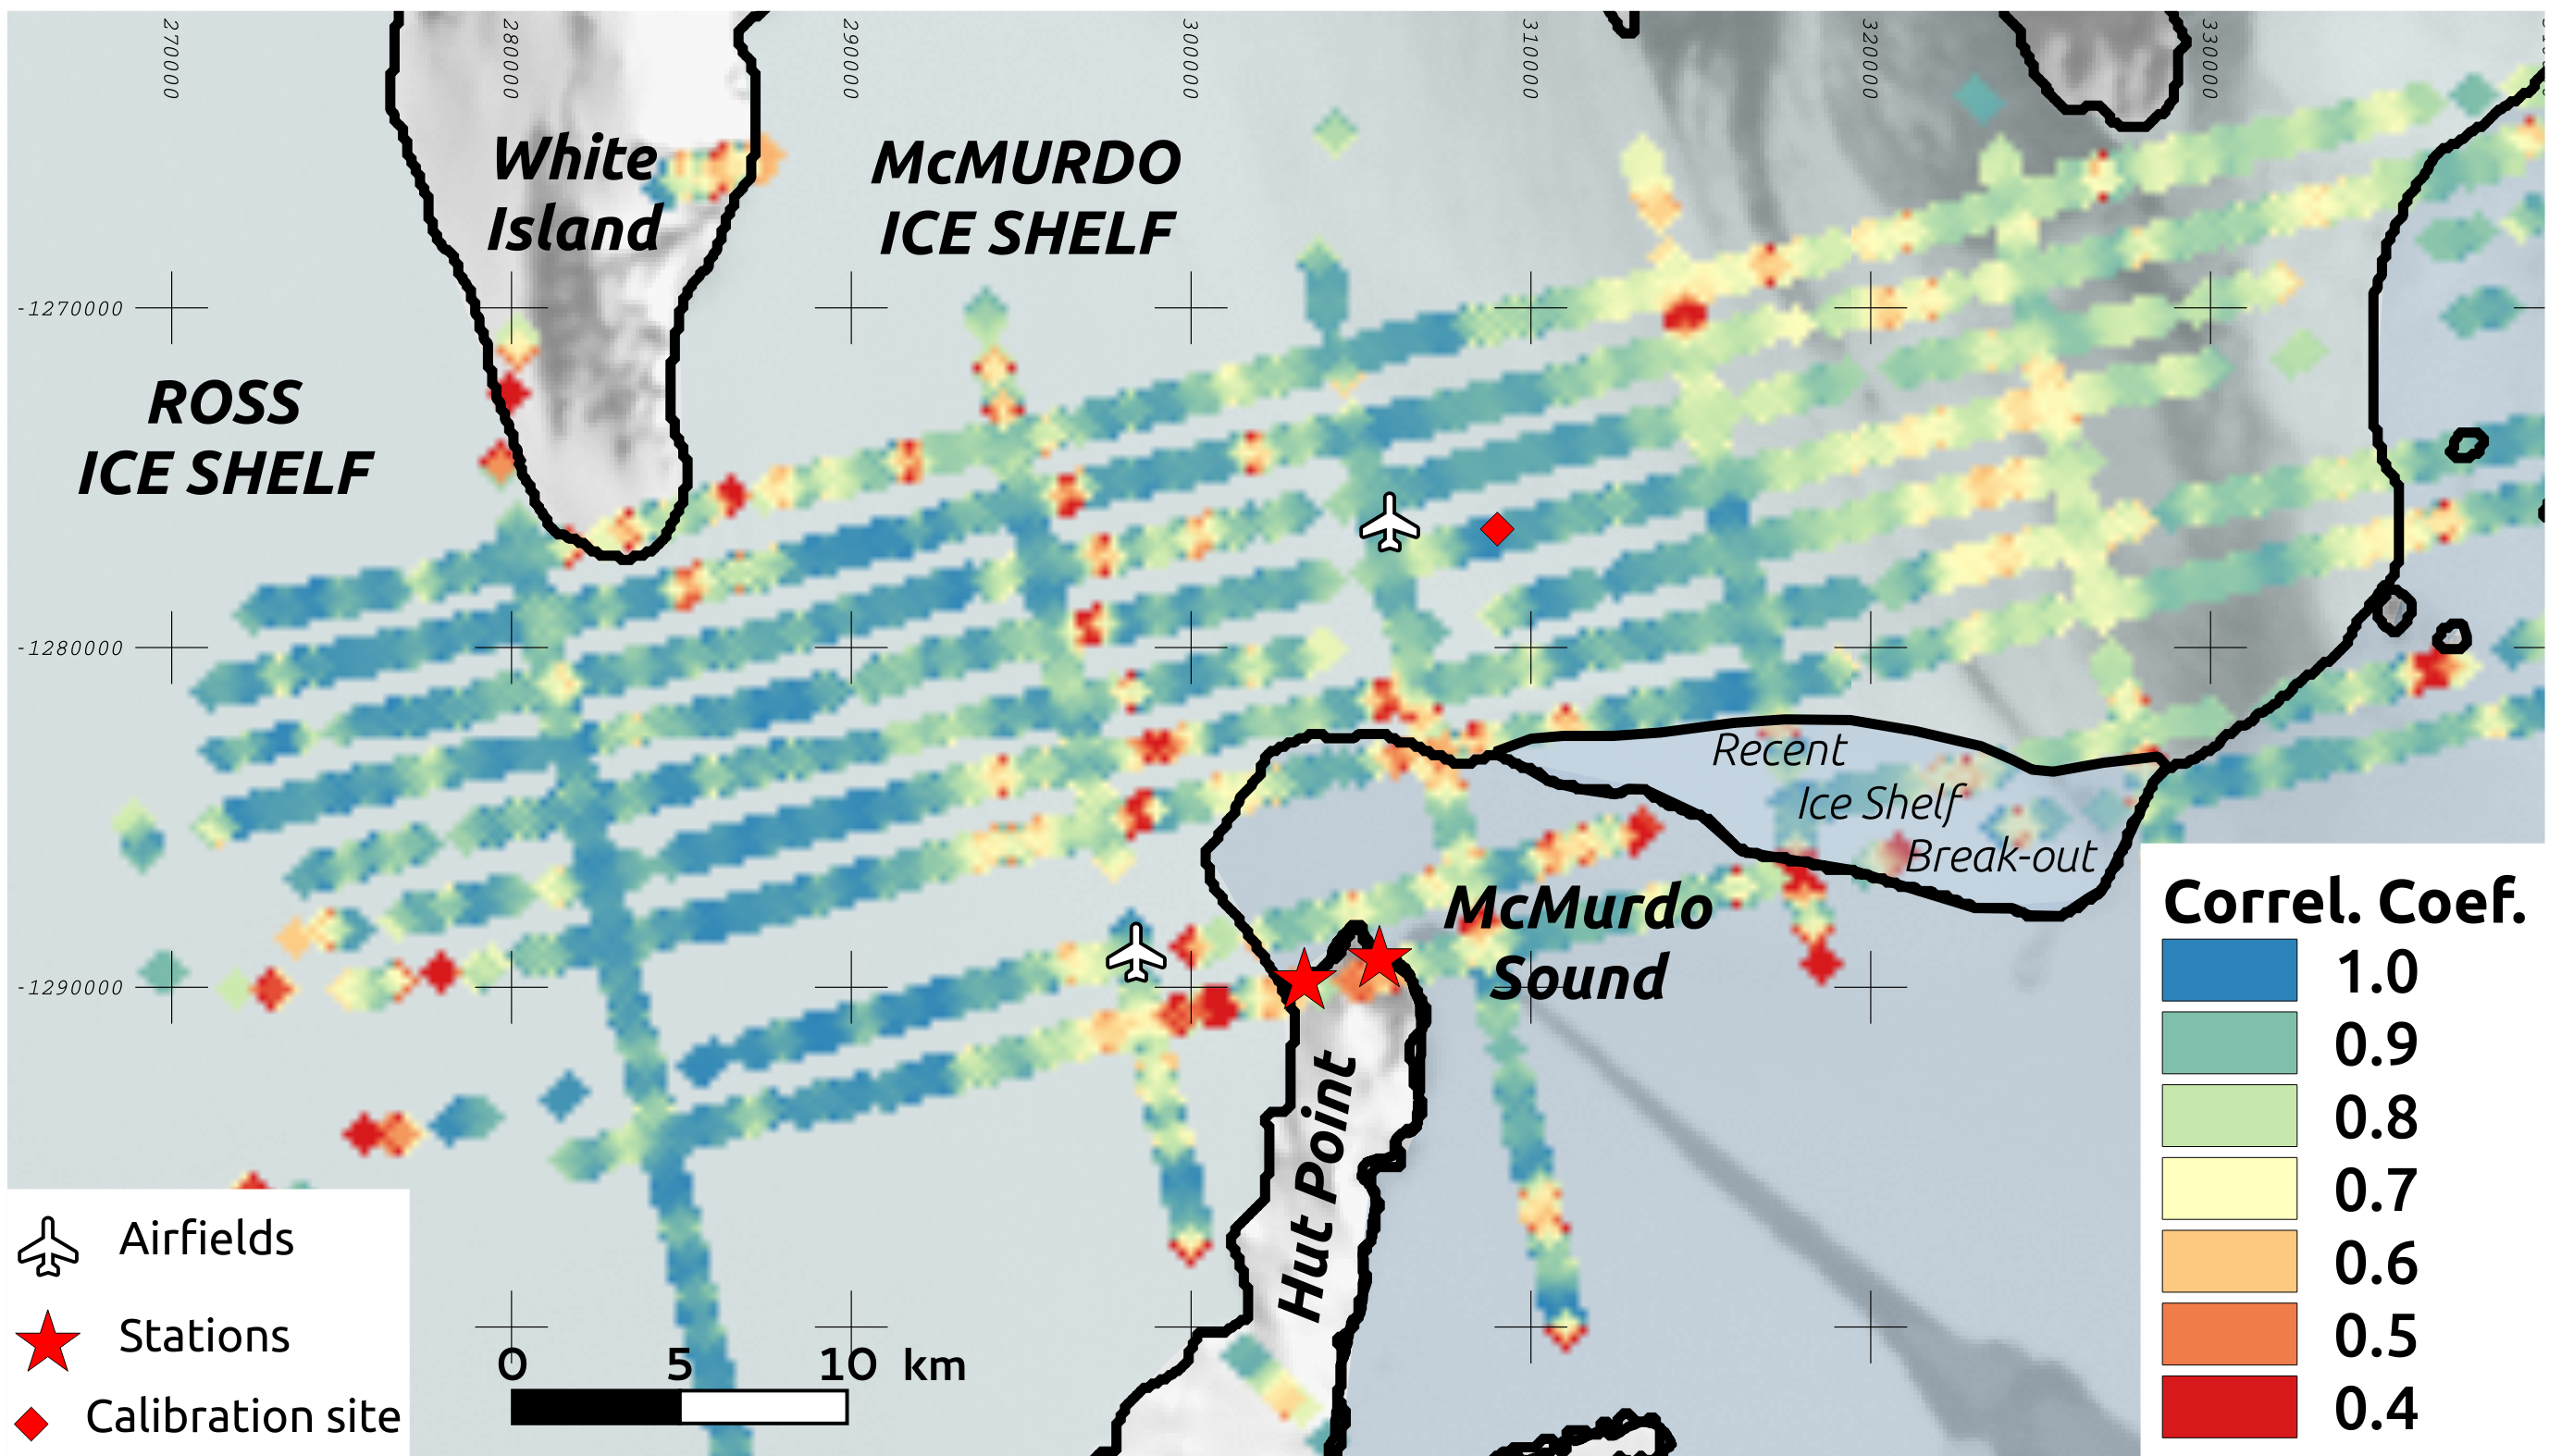
\includegraphics[width=\textwidth]{figS4}
\caption{Correlation coefficient ($\rho$) of the fit between the empirical surface echo amplitudes distribution and the theoretical HK envelope. A low $\rho$ generally means a more heterogenous surface with a higher uncertainty on the RSR-derived parameters.}
 \label{correlcoef}
 \end{figure}
 
 
  \begin{figure}
\setfigurenum{S5}  %%Change number for each figure
 \noindent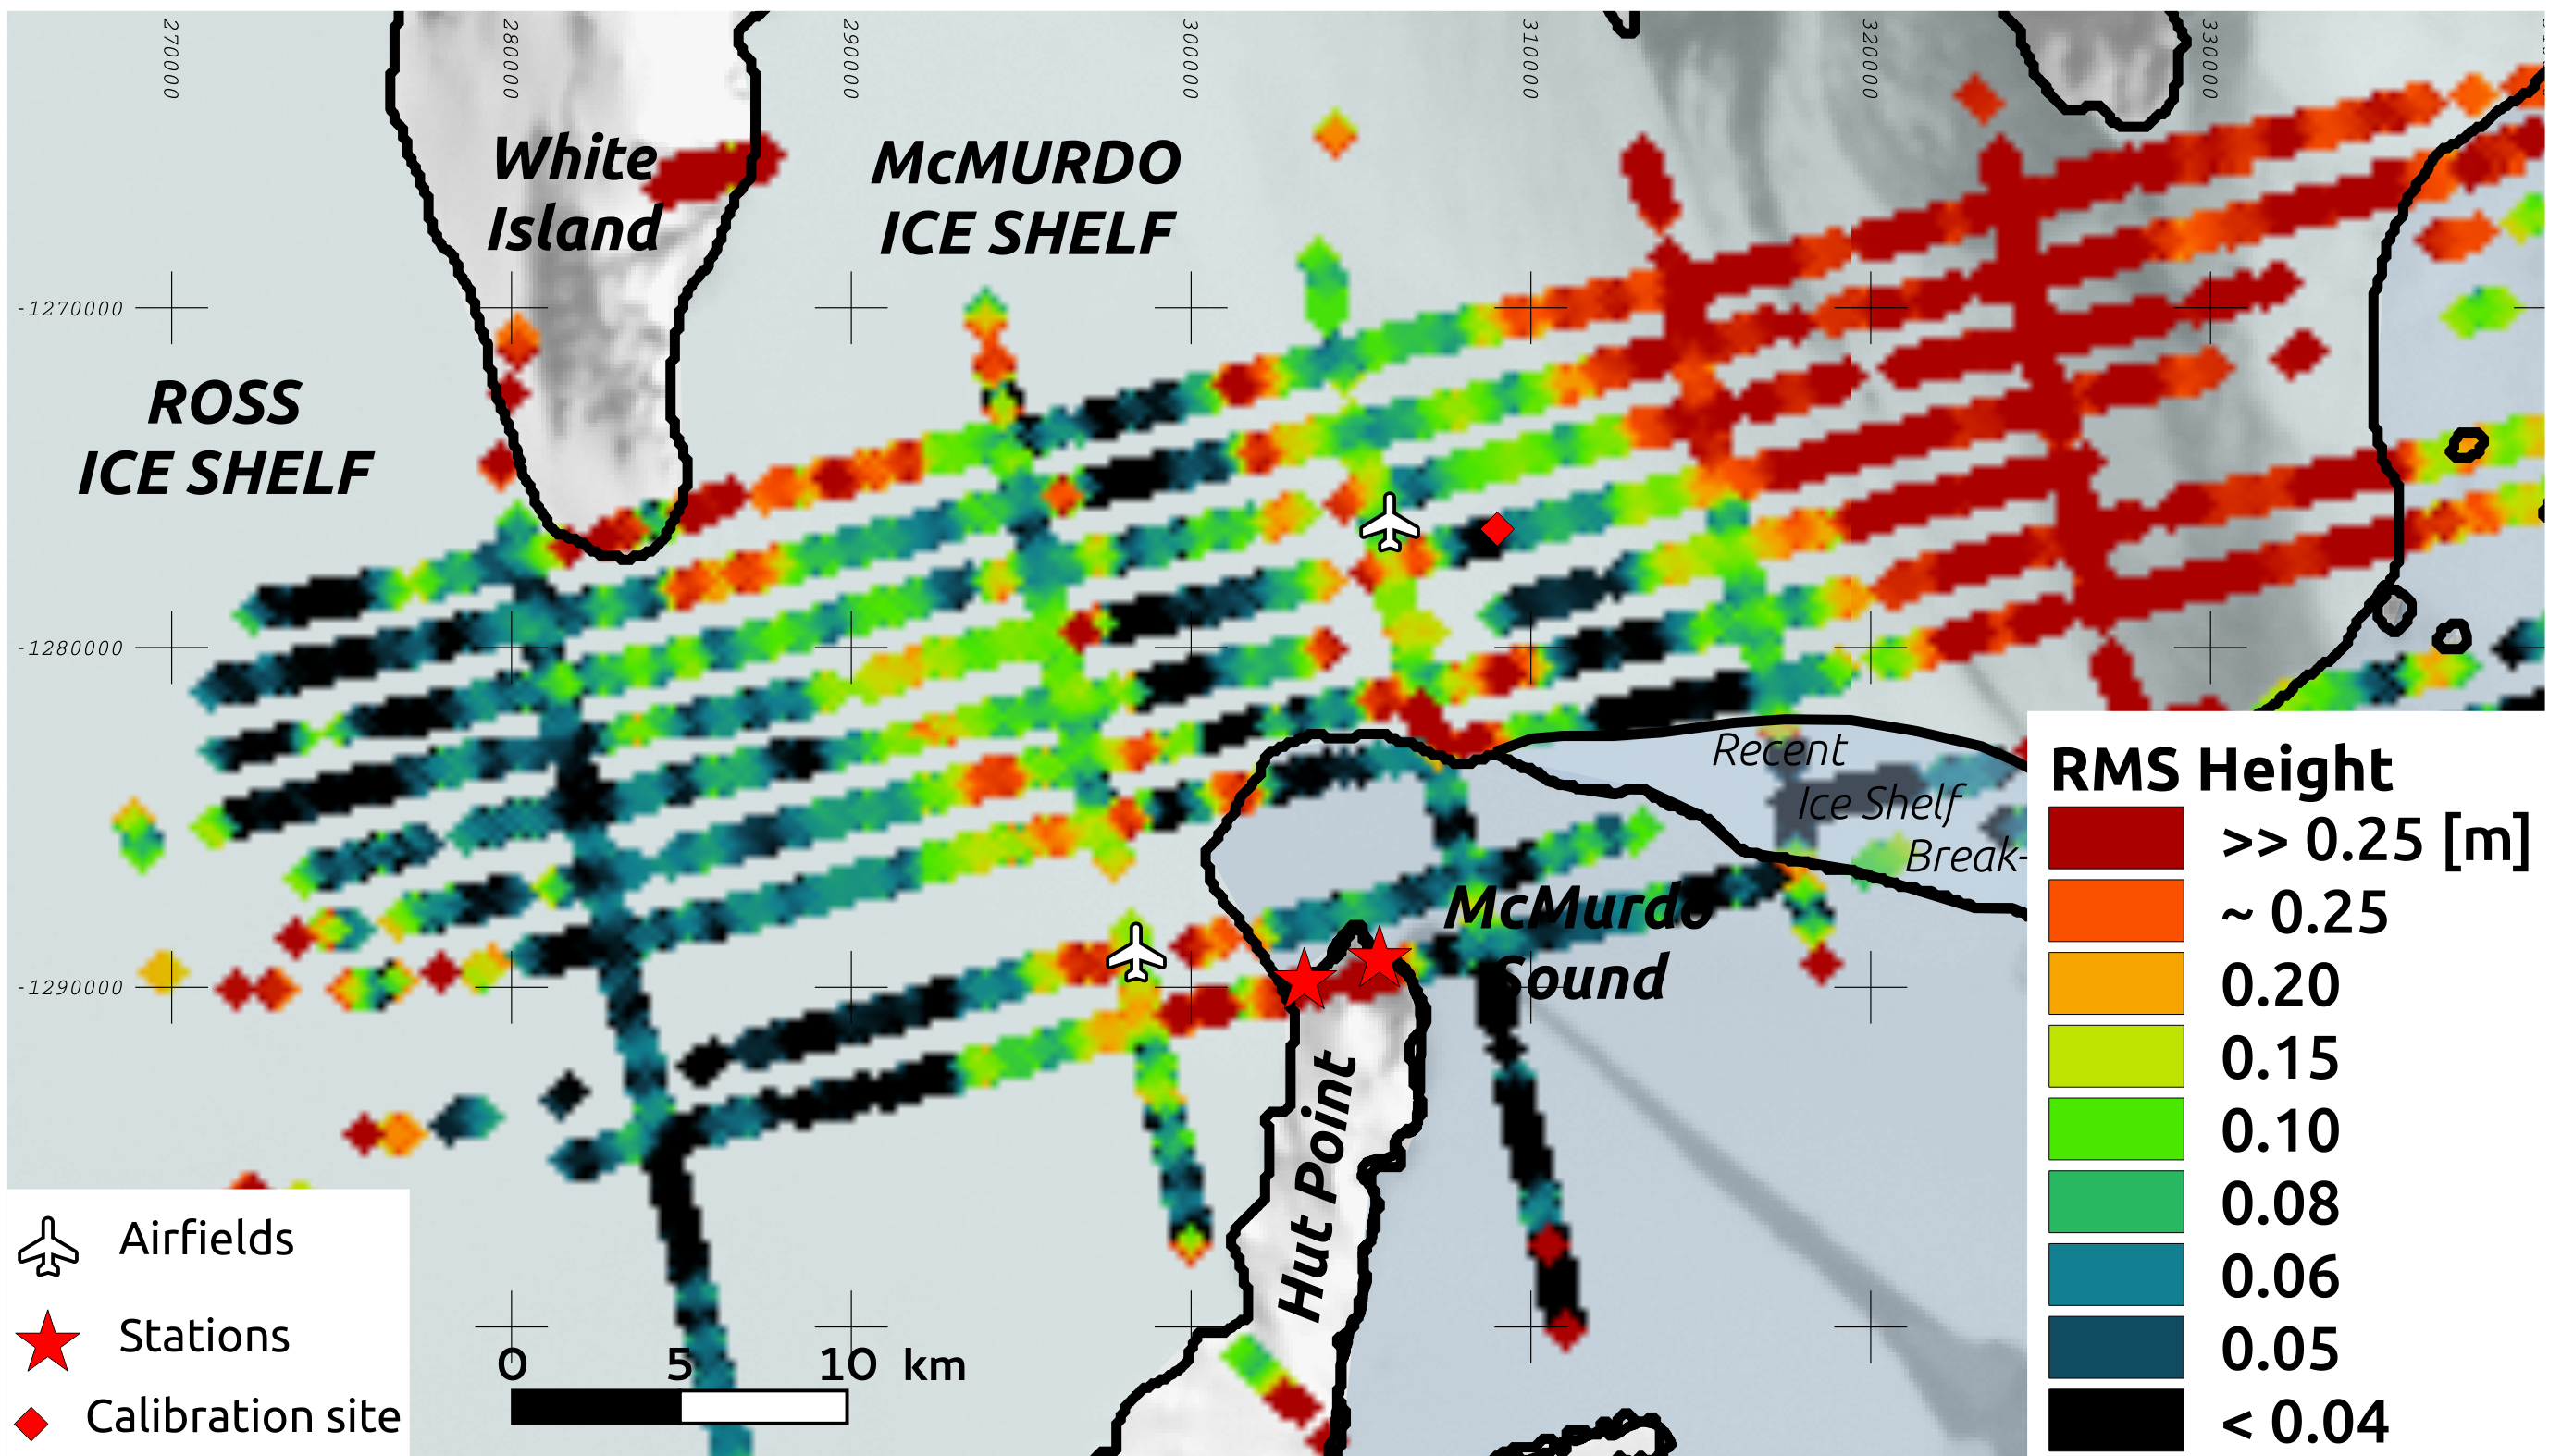
\includegraphics[width=\textwidth]{figS5}
\caption{Surface root-mean-square heights ($\sigma_h$, roughness) derived from the Small Perturbation Model. Values $> $0.25~m (5 $\%$ of the signal wavelength) are understimated. Underestimation increases with increasing roughness above this threshold.}
 \label{roughness}
 \end{figure}
 
 
  \begin{figure}
\setfigurenum{S6}  %%Change number for each figure
 \noindent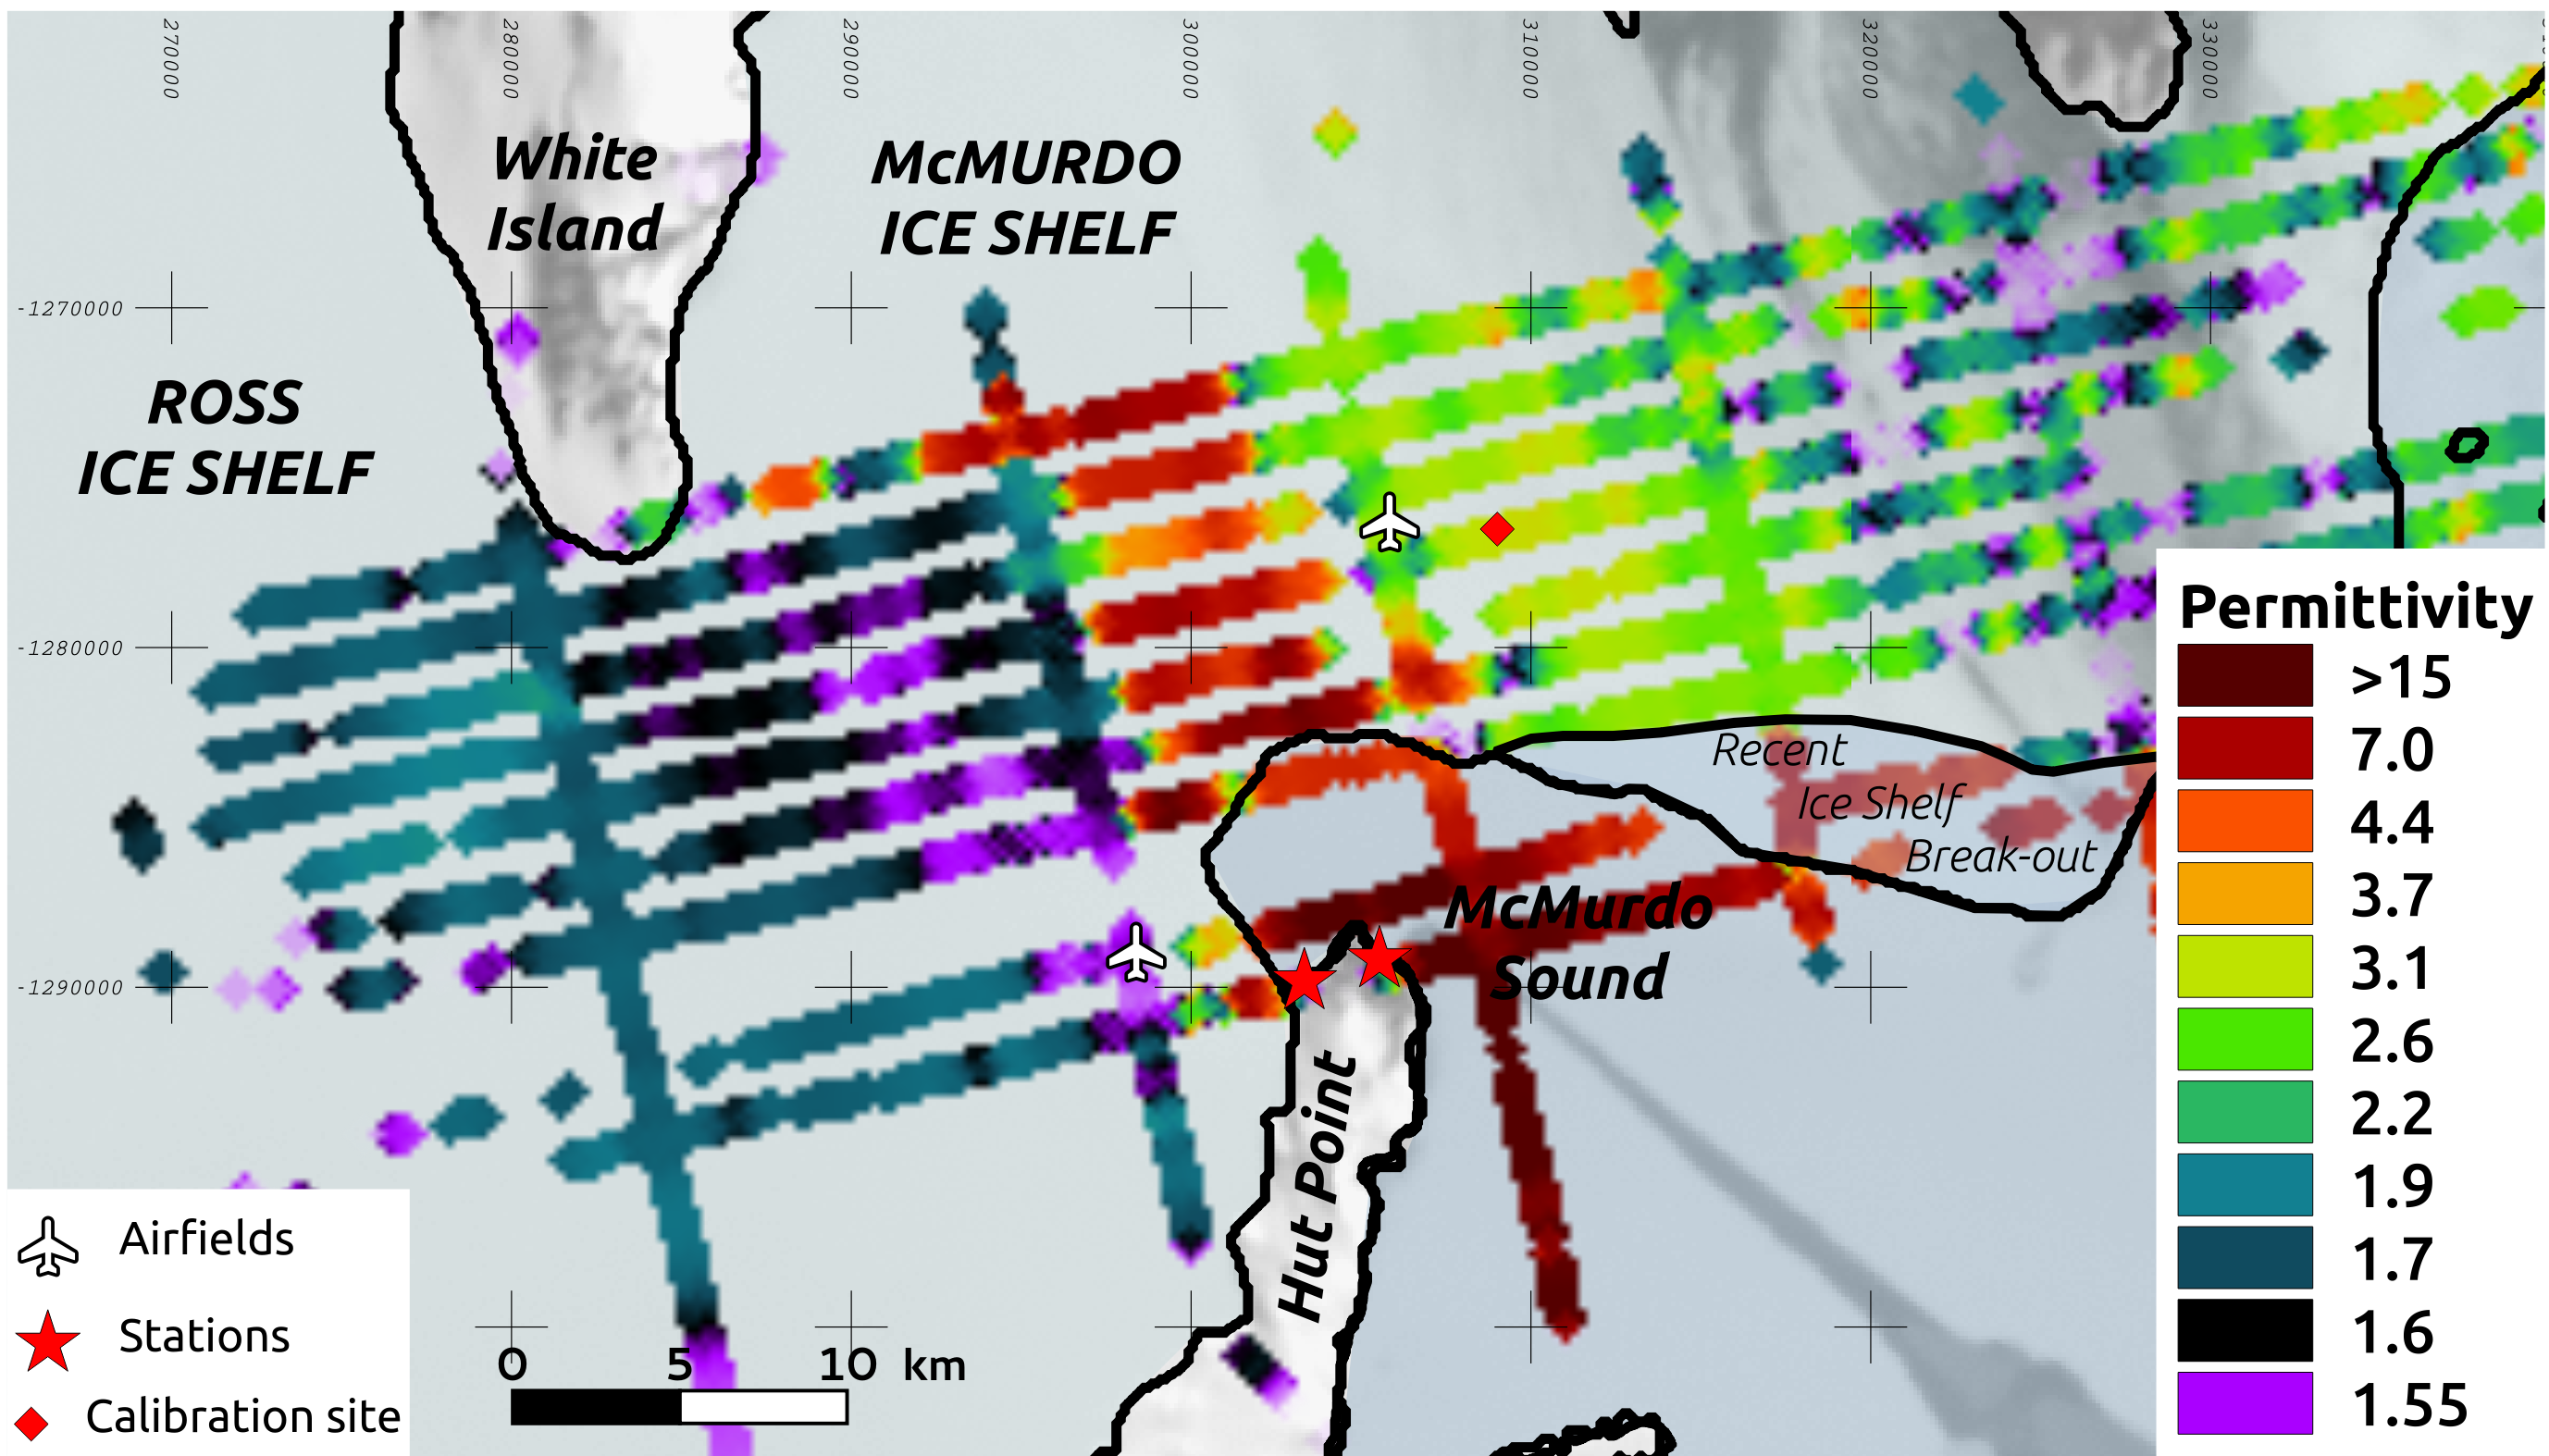
\includegraphics[width=\textwidth]{figS6}
\caption{Surface permittivity ($\epsilon$) derived from the small perturbation model. $\epsilon$ is uncertain where $\sigma_h > $0.25~m.}
 \label{permittivity}
 \end{figure}


%% ------------------------------------------------------------------------ %%
%
%  REFERENCE LIST AND TEXT CITATIONS
%
%% ------------------------------------------------------------------------ %%

%

\begin{thebibliography}{22}
\providecommand{\natexlab}[1]{#1}
\expandafter\ifx\csname urlstyle\endcsname\relax
  \providecommand{\doi}[1]{doi:\discretionary{}{}{}#1}\else
  \providecommand{\doi}{doi:\discretionary{}{}{}\begingroup
  \urlstyle{rm}\Url}\fi

\bibitem[{\textit{Frolov and Macheret}(1999)}]{Frolov-1999-ID216}
Frolov, A.~D., and Y.~Y. Macheret (1999), On dielectric propreties of dry and
  wet snow, \textit{Hydrological Processes}, \textit{13}(12-13), 1755–1760.

\bibitem[{\textit{Grima et~al.}(2014{\natexlab{a}})\textit{Grima, Blankenship,
  Young, and Schroeder}}]{Grima-2014-ID867}
Grima, C., D.~D. Blankenship, D.~A. Young, and D.~M. Schroeder
  (2014{\natexlab{a}}), Surface slope control on firn density at thwaites
  glacier, west antarctica: Results from airborne radar sounding,
  \textit{Geophysical Research Letters}, \textit{41}(19), 6787--6794,
  \doi{10.1002/2014GL061635}.

\bibitem[{\textit{Grima et~al.}(2014{\natexlab{b}})\textit{Grima, Schroeder,
  Blankenship, and Young}}]{Grima-2014-ID865}
Grima, C., D.~M. Schroeder, D.~D. Blankenship, and D.~A. Young
  (2014{\natexlab{b}}), Planetary landing-zone reconnaissance using
  ice-penetrating radar data: Concept validation in antarctica,
  \textit{Planetary and Space Science}, \textit{103}, 191--204,
  \doi{10.1016/j.pss.2014.07.018}.

\bibitem[{\textit{Jakeman}(1980)}]{Jakeman-1980-ID344}
Jakeman, E. (1980), On the statistics of k-distributed noise, \textit{Journal
  of Physics A: Mathematical and General}, \textit{13}(1), 31--48,
  \doi{10.1088/0305-4470/13/1/006}.

\bibitem[{\textit{Jakeman and Tough}(1987)}]{Jakeman-1987-ID343}
Jakeman, E., and R.~J.~A. Tough (1987), Generalized k distribution: a
  statistical model for weak scattering, \textit{Journal of the Optical Society
  of America A}, \textit{4}(9), 1764, \doi{10.1364/JOSAA.4.001764}.

\bibitem[{\textit{Kovacs et~al.}(1995)\textit{Kovacs, Gow, and
  Morey}}]{Kovacs-1995-ID697}
Kovacs, A., A.~J. Gow, and R.~M. Morey (1995), The in-situ dielectric constant
  of polar firn revisited, \textit{Cold Regions Science and Technology},
  \textit{23}(3), 245--256, \doi{10.1016/0165-232X(94)00016-Q}.

\bibitem[{\textit{Ogilvy}(1991)}]{Ogilvy-1991-ID817}
Ogilvy, J.~A. (1991), \textit{Theory of Wave Scattering From Random Rough
  Surfaces}, CRC Press.

\bibitem[{\textit{Thorsos and Jackson}(1989)}]{Thorsos-1989-ID713}
Thorsos, E.~I., and D.~R. Jackson (1989), The validity of the perturbation
  approximation for rough surface scattering using a gaussian roughness
  spectrum, \textit{The Journal of the Acoustical Society of America},
  \textit{86}, 261--277, \doi{10.1121/1.398342}.

\bibitem[{\textit{Ulaby et~al.}(1981)\textit{Ulaby, Moore, and
  Fung}}]{Ulaby-1981-ID816}
Ulaby, F.~T., R.~K. Moore, and A.~K. Fung (1981), \textit{Microwave Remote
  Sensing: Active and Passive}, vol. 1-3, Addison-Wesley, Advanced Book
  Program, Reading, Massachusetts.

\end{thebibliography}


\end{document}